\section{Introduction}

\subsection{Problem statement}
During a cricket tournament the same questions come up after every match: \emph{can team X still reach the
top four, what does it need, and who are its real rivals?} Answering them needs several kinds of knowledge at
once: match results, the points they award, net run rate (NRR), the tournament's tie-break order, the number
of qualifying places and the fixtures still to be played. General-purpose chatbots routinely get these
calculations wrong or invent standings, and a plain points table cannot explain \emph{why} a team is or is not
eliminated.

QualifyPath-KG represents results, fixtures and the tournament's rules explicitly in a knowledge graph,
derives standings and qualification status by reasoning, and lets an LLM answer natural-language questions
only from facts retrieved from that graph, with every claim traceable to stored or inferred knowledge.

\subsection{Why a knowledge graph}
Qualification depends on connected facts: teams play matches, matches produce results, results award points
and NRR, tie-break rules decide standings, and the remaining fixtures decide what is still possible. A
knowledge graph keeps these relationships and the rules explicit, so facts that are never stored --- a team's
points, its maximum reachable total, whether it is eliminated --- can be inferred and explained
\citep{hogan2021knowledge}. Multi-hop paths (team $\rightarrow$ remaining match $\rightarrow$ opponent
$\rightarrow$ standing) show exactly what each team needs. Because the rules are data, the same model works for
any league-stage tournament. A relational database could store the results, but would hide the reasoning in
application code; an LLM alone has no reliable access to this season's facts at all (Section~\ref{sec:eval}).

\subsection{Scope and snapshot}
The graph models the IPL~2026 league stage as a \emph{snapshot after match~39} (27~April~2026): matches 1--39
have results and matches 40--70 are scheduled fixtures. The snapshot is where the dataset's match table and
official points table stop, it gives genuine remaining fixtures to reason about, and it lets us validate every
derived standing against the published table.

\subsection{Contributions}
\begin{itemize}
  \item An OWL ontology (\statClasses{} classes, \statObjProps{} object and \statDataProps{} datatype properties,
        five reasoning constructs) and a cleaned, validated RDF knowledge graph of the IPL~2026 league stage.
  \item Eleven SPARQL queries, seven SPARQL Update rules (points, NRR, reachable points, qualification status,
        position) and three demonstrated symbolic inferences, in Python and in GraphDB.
  \item A multi-hop reasoner (Option~C) that returns complete, provenance-labelled reasoning paths and is
        evaluated against independently computed ground truth.
  \item A KG-grounded question-answering application with evidence display, refusal on insufficient
        evidence, and a 10-question comparison against the same LLM without the graph.
\end{itemize}

\begin{figure}[H]
\centering
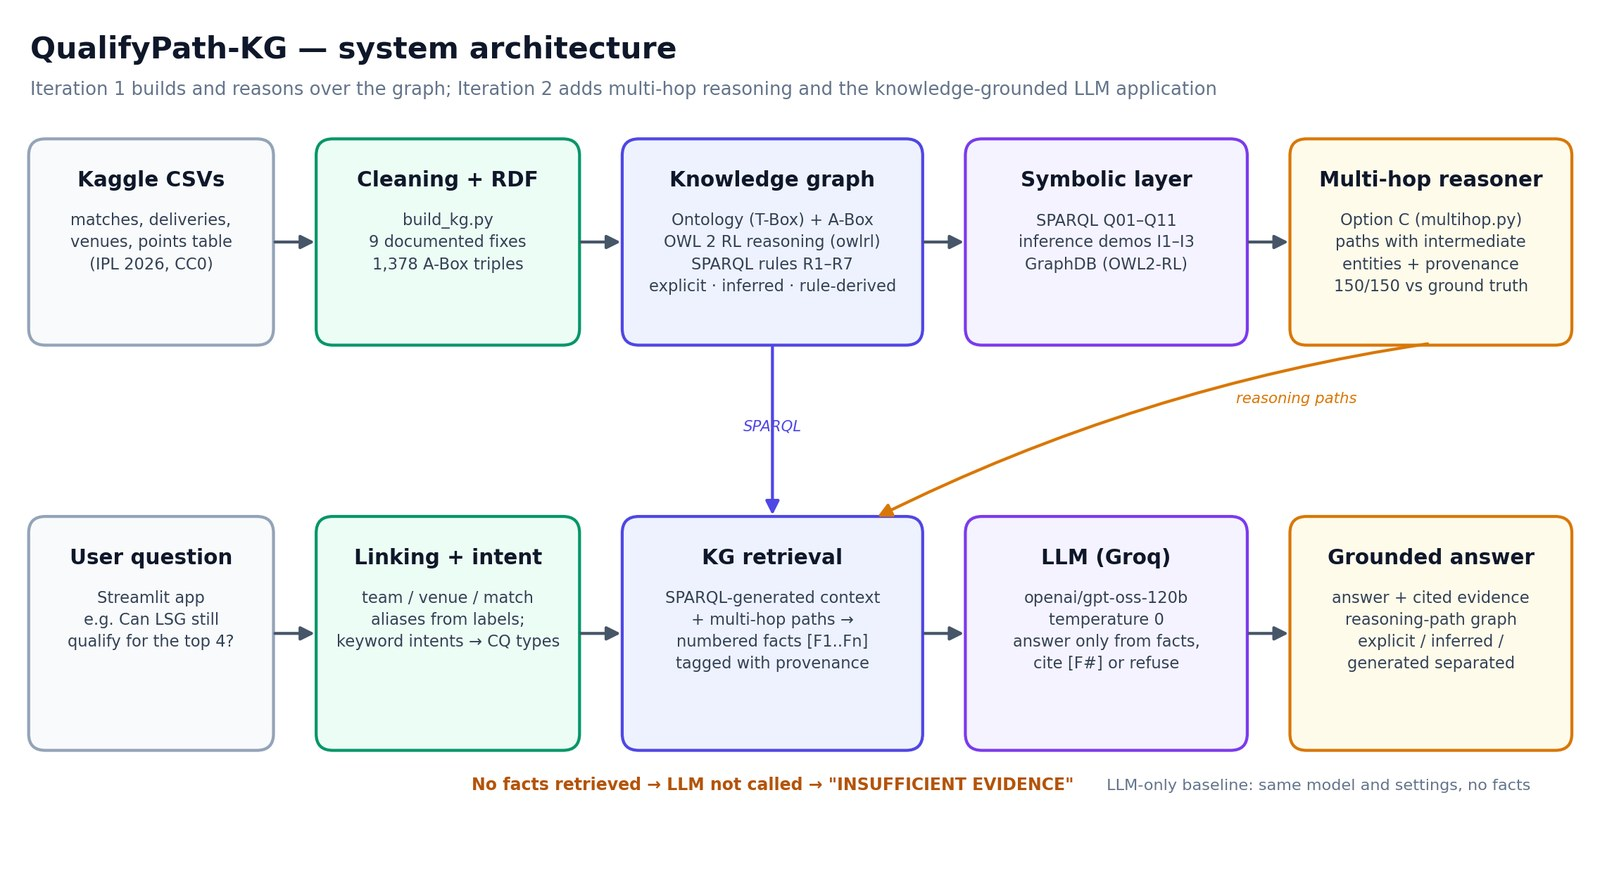
\includegraphics[width=\linewidth]{figures/architecture.jpg}
\caption{End-to-end architecture. Top: Iteration~1 knowledge graph and symbolic layer, plus the Iteration~2
multi-hop reasoner. Bottom: the question-answering pipeline.}
\label{fig:architecture}
\end{figure}
